\documentclass[12pt,letterpaper,twoside]{hmcpset}
\usepackage[margin=1in]{geometry}
\usepackage{graphicx}
\usepackage{commons}
\usepackage{ulem}
\usepackage{tikz}
\usetikzlibrary{trees}

% info for header block in upper right hand corner
\name{Zachary Seymour}
\class{CS 520}
\assignment{Assignment 3}
\duedate{November 22, 2013}

\begin{document}
\begin{problem}[1]
 Consider the following stream of memory word addresses directed at the cache. Assume that the memory is word addressable, and the total cache capacity is 64 words. Further assume that the cache is 2-way set-associative, the cache line size is 8 words and the LRU replacement policy is used. 
\[5, 7, 1, 12, 34, 39, 65, 3, 107\]
For each of these accesses, indicate whether it is a cache hit or a cache miss, show how you computed the cache index, and depict the contents of the cache after every access. You do not have to show the tag bits, only show the addresses of the cached data.
\end{problem}

\begin{solution}
 Since our total size is 64 words and each cache line is 8 words, we have 8 cache entries and thus four sets in a 2-way set-associative cache.  Thus, we proceed with the stream of addresses
 \begin{itemize}
  \item 5
  \begin{itemize}
  \item Cache Index: $5 \mod{4} = 1$
  \item Cache Miss
  \item Cache contents
  
  \begin{tabular}{ccc}
    Set & Data & Data\\
    0 &  & \\
    1 & 5 & \\
    2 &  & \\
    3 &  & 
  \end{tabular}
  \end{itemize}
   \item 7
  \begin{itemize}
  \item Cache Index: $7 \mod{4} = 3$
  \item Cache Miss
  \item Cache contents
  
  \begin{tabular}{ccc}
    Set & Data & Data\\
    0 &  & \\
    1 & 5 & \\
    2 &  & \\
    3 & 7 & 
  \end{tabular}
  \end{itemize}
   \item 1
  \begin{itemize}
  \item Cache Index: $1 \mod{4} = 1$
  \item Cache Miss
  \item Cache contents
  
  \begin{tabular}{ccc}
    Set & Data & Data\\
    0 &  & \\
    1 & 5 & 1\\
    2 &  & \\
    3 & 7 & 
  \end{tabular}
  \end{itemize}
 \item 12
  \begin{itemize}
  \item Cache Index: $12 \mod{4} = 0$
  \item Cache Miss
  \item Cache contents
  
  \begin{tabular}{ccc}
    Set & Data & Data\\
    0 & 12 & \\
    1 & 5 & 1\\
    2 &  & \\
    3 & 7 & 
  \end{tabular}
  \end{itemize}
\item 34
  \begin{itemize}
  \item Cache Index: $34 \mod{4} = 2$
  \item Cache Miss
  \item Cache contents
  
  \begin{tabular}{ccc}
    Set & Data & Data\\
    0 & 12 & \\
    1 & 5 & 1\\
    2 & 34 & \\
    3 & 7 & 
  \end{tabular}
  \end{itemize}
  \item 39
  \begin{itemize}
  \item Cache Index: $39 \mod{4} = 3$
  \item Cache Miss
  \item Cache contents
  
  \begin{tabular}{ccc}
    Set & Data & Data\\
    0 & 12 & \\
    1 & 5 & 1\\
    2 & 34 & \\
    3 & 7 & 39
  \end{tabular}
  \end{itemize}
  \item 65
  \begin{itemize}
  \item Cache Index: $65 \mod{4} = 1$
  \item Cache Miss
  \item Cache contents
  
  \begin{tabular}{ccc}
    Set & Data & Data\\
    0 & 12 & \\
    1 & 65 & 1\\
    2 & 34 & \\
    3 & 7 & 39
  \end{tabular}
  \end{itemize}
  \item 3
  \begin{itemize}
  \item Cache Index: $3 \mod{4} = 3$
  \item Cache Miss
  \item Cache contents
  
  \begin{tabular}{ccc}
    Set & Data & Data\\
    0 & 12 & \\
    1 & 65 & 1\\
    2 & 34 & \\
    3 & 3 & 39
  \end{tabular}
  \end{itemize}
  \item 107
  \begin{itemize}
  \item Cache Index: $107 \mod{4} = 3$
  \item Cache Miss
  \item Cache contents
  
  \begin{tabular}{ccc}
    Set & Data & Data\\
    0 & 12 & \\
    1 & 65 & 1\\
    2 & 34 & \\
    3 & 3 & 107
  \end{tabular}
  \end{itemize}
 \end{itemize}

\end{solution}

\begin{problem}[2]
 Consider a system with physically-addressed caches, and assume that 40-bit virtual addresses and 32-bit physical addresses are used, and the memory is byte-addressable.  Further assume that the cache is 4-way set-associative, the cache line size is 64 Bytes and the total size of the cache is 64 KBytes.  Answer the following questions, providing adequate explanations in all cases:
\end{problem}

\begin{problem}[2a]
What should be the minimum page size in this system to allow for the overlap of the TLB access and the cache access?
\end{problem}

\begin{solution}
 In this scenario, we have 1024 cache entries and thus 256 cache sets, which will require 7 bits for indexing.  Further, our virtual address space is $2^{40} = 128$ GB  We also know that we have $40 - (7+2)= 31$ bits remaining for our page number, so we have $2^{31}$ pages with $2^9$ bits or 64 bytes as our minimum page size. 
\end{solution}

\begin{problem}[2b]
 Repeat part (a) assuming that the cache associativity is increased to 8. Assume that the total cache size and the cache line size remain the same.
\end{problem}

\begin{solution}
 Here now, we still have 1024 cache entries, but only 128 sets, so we need 6 bits to index the cache.  So, our page number increases to 32 bits, and we then have $2^8$ bits or 32 bytes for our page size.
\end{solution}

\begin{problem}[2c]
 Assuming that the memory page size in this system is as calculated in your answer to Part (b), compute the total size of the page table in bytes.  Assume that a simple linear page table is used and only the page translation information is stored in each entry, with no additional bits.
\end{problem}

\begin{solution}
 If we allocate $6+2=8$ bits for the page offset, then we have remaining 32 bits for the virtual page number, so we have $2^{32}$ pages at 32.  We need $32+24=56$ bits per page, so the total size of the page table is 28 GB.
\end{solution}


\begin{problem}[2d]
 Repeat part (b) assuming that the OS can guarantee that the two least significant bits of the page number would not change during the address translation. 
\end{problem}

\begin{solution}
 In this case, we use 29 bits for our page number, so we have $2^{11}$ bits or 256 bytes as our page size.
\end{solution}

\begin{problem}[2e]
 Assume that the OS needs to establish a mapping for the virtual page number 52356 (expressed in decimal). List some possible frame numbers in the physical memory where this page can be mapped to support the OS guarantee described in part (d).
\end{problem}

\begin{solution}
 $52356 = 0b1100110010000100$, so 52364, 52236, or 52748, for example, as long as the last two bits are still 00.
\end{solution}

\begin{problem}[3]
 Consider the use of multi-level hot-cold bits in implementing a replacement algorithm for a set-associative cache with $2^p$ ways and $S$ sets. This is an approximation of the LRU policy that marks the most recently assessed way as hot, and the other one as cold (for a 2-way set-associative cache). This mechanism can be extended to more than two ways by providing multiple levels of hot-cold bits. For example, for a 4-way cache the victim is determined as the cold way of the cold pair.
\end{problem}

\begin{problem}[3a]
 What is the total number of hot-cold bits for each set in this cache?
\end{problem}

\begin{solution}
 We can model the multi-level hot-cold bits as a binary tree, where the height corresponds to the log of the associativity, minus the root node, because a cache of associativity one will not need a hot-cold bit.  So, the number of bits per set is $2^{p+1} - 2$.
\end{solution}

\begin{problem}[3b]
 What is the total number of hot-cold bits in the cache?
\end{problem}

\begin{solution}
 The total number of hot-cold bits in the whole cache is equal to the number per set times the number of sets, so we have $S\left(2^{p+1} - 2\right)$.
\end{solution}

\begin{problem}[3c]
 Assume that $p = 2$ and accesses to a specific set result to the following ways in sequence and no misses occur:

	Way 0, Way 3, Way 2, Way 0, Way 1, Way 1, Way 2, Way 3, Way 2, Way 0

At the end of the fifth access in this sequence (to Way 1), what are the settings of the hot-cold bit?  Do they point to the same victim that would have been selected by a true-LRU algorithm?
\end{problem}

\begin{solution}
Say we number our bits as such:

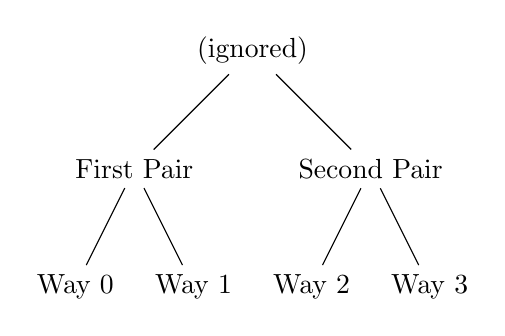
\begin{tikzpicture}[level distance=1.5cm,
  level 1/.style={sibling distance=3cm},
  level 2/.style={sibling distance=1.5cm}]
  \node {(ignored)}
    child {node {First Pair}
      child {node {Way 0}}
      child {node {Way 1}}
    }
    child {node {Second Pair}
    child {node {Way 2}}
      child {node {Way 3}}
    };
\end{tikzpicture}

\begin{tabular}{|l|l|}\hline
Bit & Hot/Cold\\\hline
First Pair & \sout{1} \sout{0} 1\\\hline
Second Pair & \sout{0} \sout{1} 0\\\hline
Way 0 & \sout{1} 0\\\hline
Way 1 & \sout{0} 1\\\hline
Way 2 & \sout{0} 1\\\hline
Way 3 & \sout{0} \sout{1} 0\\\hline
\end{tabular}

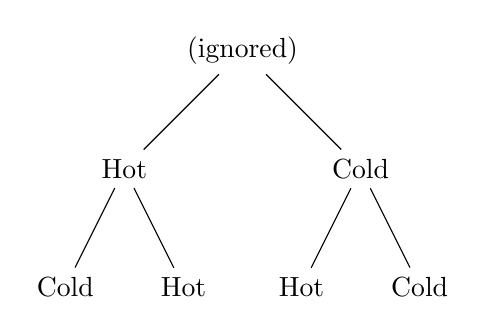
\begin{tikzpicture}[level distance=1.5cm,
  level 1/.style={sibling distance=3cm},
  level 2/.style={sibling distance=1.5cm}]
  \node {(ignored)}
    child {node {Hot}
      child {node {Cold}}
      child {node {Hot}}
    }
    child {node {Cold}
    child {node {Hot}}
      child {node {Cold}}
    };
\end{tikzpicture}

The victim pointed to then is Way 3, which is indeed the least recently used way as well.

\end{solution}

\begin{problem}[3d]
 Repeat Part (c), assuming that the all accesses shown in the sequence given in Part (c) have been completed with the last access being made to Way 0.
\end{problem}

\begin{solution}
 \begin{tabular}{|l|l|}\hline
Bit & Hot/Cold\\\hline
First Pair & \sout{1} \sout{0} \sout{1} \sout{0} 1\\\hline
Second Pair & \sout{0} \sout{1} \sout{0} \sout{1} 0\\\hline
Way 0 & \sout{1} \sout{0} 1\\\hline
Way 1 & \sout{0} \sout{1} 0\\\hline
Way 2 & \sout{0} \sout{1} \sout{0} 1\\\hline
Way 3 & \sout{0} \sout{1} \sout{0} \sout{1} 0\\\hline
\end{tabular}

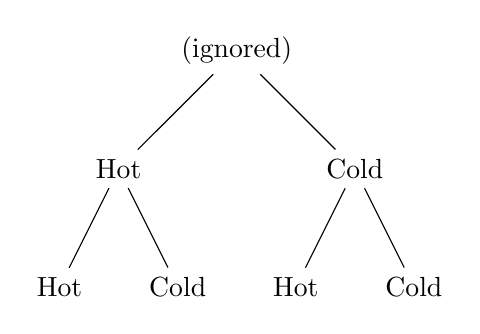
\begin{tikzpicture}[level distance=1.5cm,
  level 1/.style={sibling distance=3cm},
  level 2/.style={sibling distance=1.5cm}]
  \node {(ignored)}
    child {node {Hot}
      child {node {Hot}}
      child {node {Cold}}
    }
    child {node {Cold}
    child {node {Hot}}
      child {node {Cold}}
    };
\end{tikzpicture}

The victim pointed to then is again Way 3; however, now the least recently used way is Way 1.
\end{solution}


\end{document}
